%%%%%%%%%%%%%%%%%%%%%%%%%%%%%%%%%%%%%%%%%%%%%%%%%%%%%%%%%%%%%%%%%%%
%%% Documento LaTeX 																						%%%
%%%%%%%%%%%%%%%%%%%%%%%%%%%%%%%%%%%%%%%%%%%%%%%%%%%%%%%%%%%%%%%%%%%
% Título:		Introducción
% Autor:  	Ignacio Moreno Doblas
% Fecha:  	2014-02-01, actualizado 2019-11-11
% Versión:	0.5.0
%%%%%%%%%%%%%%%%%%%%%%%%%%%%%%%%%%%%%%%%%%%%%%%%%%%%%%%%%%%%%%%%%%%
% !TEX root = A0.TFG.tex

\chapterbegin{Análisis inicial del problema}
\minitoc


Para alcanzar el objetivo de este proyecto se va a desarrollar un videojuego del género de concursos, en el que el jugador tendrá que resolver una serie de pruebas de diferentes categorías. En el desarrollo de videojuegos se suele crear un Documento de Diseño de Juego (GDD por sus siglas en inglés) de forma previa al inicio del desarrollo. En éste se documentan todas las ideas y planificaciones para tener en cuenta durante el desarrollo del videojuego, incluyendo personajes, historia, mecánicas, público objetivo o plataforma. 

Para el desarrollo de este proyecto también se ha creado un GDD, que se encuentra añadido a esta memoria en el apéndice \ref{sec:apendice:GDD}.

Este videojuego es ante todo un juego serio, es decir, su principal propósito no es el de entretener, si no el de permitir al jugador entrenar sus habilidades cognitivas. Eso no quiere decir que el juego no contenga una parte lúdica destinada a entretener al usuario y hacer el juego divertido. En este caso, el videojuego estará ambientado en un plató de televisión para concursos similar al mostrado en la figura \ref{fig:AI_atrapaMillon}, tomando una estructura similar a dichos concursos. 

El jugador se encontrará en el centro de un plató, rodeado de público y con una pantalla en frente en la que se le presentarán pruebas y preguntas. Dependiendo del resultado de cada prueba, el jugador sumará puntos a su marcador, que servirá para valorar su sesión de entrenamiento al final del juego. A pesar de utilizar un sistema de puntuación, no se trata de un juego puramente competitivo, la función de los puntos es tratar de animar y recompensar el jugador.

\begin{figure}
  \centering
    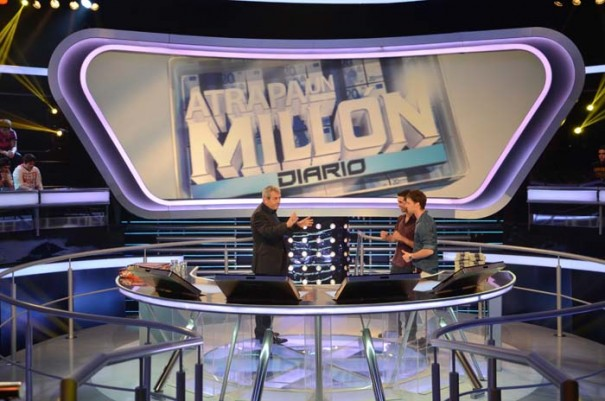
\includegraphics[width=0.5\textwidth]{03.EstudioProblema/02.AnalisisInicial/00.Figuras/01.atrapa_un_millon.jpg}
    \caption{Plató del programa de televisión 'Atrapa un millón'. \cite{AI_img_atrapaMillon}}
    \label{fig:AI_atrapaMillon}
\end{figure}

\section{Pruebas}
Las pruebas están diseñadas para estimular determinadas habilidades cognitivas ya vistas en el apartado \ref{sec:estadoArte:cognicion} a partir de los juegos y mecánicas que se utilizan en entrenamientos cognitivos actuales como los presentados en la sección \ref{sec:estadoArte:ejerciciosBrainTraining}.
Estas pruebas se pueden agrupar en cinco categorías dependiendo principalmente del tipo de habilidades cognitivas que ejercitan.



\subsection{Motricidad}

En esta categoría se incluyen las pruebas que se centran en entrenar la capacidad de movimiento, reflejos motores y la consciencia de la posición del cuerpo de uno mismo en el espacio. Estas pruebas requieren del movimiento del jugador por lo que dependiendo de las capacidades individuales de los usuarios pueden resultar más o menos complejas. 

Se busca, además, activar físicamente al jugador, no solo para mantener una buena salud cognitiva, si no también física.

\subsubsection{Baile}

La música es uno de los estímulos más potentes para el ser humano, por lo que en este caso se pretende usarla para animar al jugador y hacer que se mueva al ritmo de canciones conocidas por el mismo. El jugador tendrá que realizar una serie de movimientos con sus brazos y piernas al ritmo de la música. 

Estos movimientos requerirán posicionar una o varias extremidades en lugares concretos relativos al usuario, realizar movimientos de un punto a otro como se ve en la figura \ref{fig:AI_baile}, o se dejará libertad para que el usuario elija sus propios movimientos durante un tiempo. Con esto último se pretende que el usuario se deje llevar por los sentimientos evocados por las canciones, sirviendo como ejercicio de ocio y expresión emocional.

\begin{figure}
  \centering
    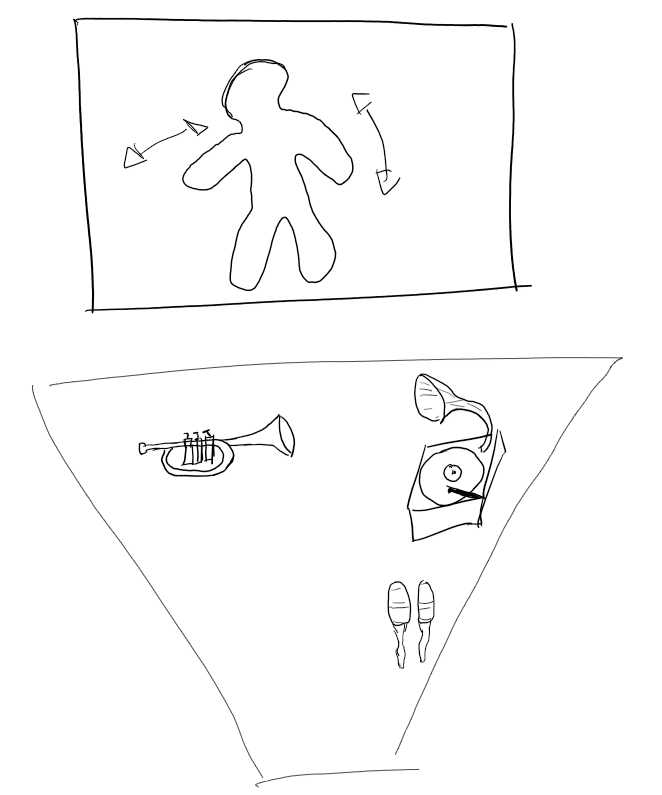
\includegraphics[width=0.5\textwidth]{03.EstudioProblema/02.AnalisisInicial/00.Figuras/02.baile.png}
    \caption{Boceto del escenario para la prueba de baile.}
    \label{fig:AI_baile}
\end{figure}

\subsubsection{Figuras}

De forma similar a la prueba anterior, el jugador debe adquirir una serie de poses concretas, aunque en este caso se realizará si música. Eliminando la música se obtiene una prueba que puede ser menos atractiva para el usuario, pero que permite añadir complejidad a las poses y movimientos a ejecutar, puesto que no hay un ritmo que seguir y el usuario está en un estado más calmado. De esta forma el jugador puede tomarse el tiempo que necesite antes y después de cada figura.


\subsubsection{Parada}

Esta prueba se basa en las pruebas anteriores, pero añadiendo un modificador para entrenar los reflejos del jugador. Durante la prueba el jugador deberá realizar una serie de movimientos amplios y continuos, buscando realizar movimientos fuera del rango usual para evitar la pérdida de flexibilidad en las articulaciones. Cuando reciba una señal, deberá detener el movimiento de inmediato y mantener la posición hasta que se dé la siguiente señal para continuar el movimiento.

\subsubsection{Objetivos}

La prueba de objetivos se enfoca en los reflejos y la capacidad del jugador de conocer y entender la posición de sus extremidades en el espacio. En la prueba una serie de objetivos irán apareciendo en el campo visual del jugador. Estos objetivos se moverán desde el frente del jugador hacia él y este deberá tocarlos con sus manos para hacerlos desaparecer.



\subsection{Memoria}

Esta categoría trata de entrenar la memoria a largo plazo del jugador, para ello utiliza los dos sentidos más fuertes y que provocan recuerdos más arraigados en la memoria: la visión y el oído. 

\subsubsection{Canción}

Esta prueba utiliza la música para hacer recordar al jugador y evocar memorias que pueda haber asociado a la canción. Para ello es importante que la canción sea conocida por el usuario, por lo que es muy importante tener en mente el público objetivo del videojuego, en este caso, personas mayores. 
Durante el desarrollo de la prueba se presenta al jugador la canción y este tendrá que averiguar el autor y nombre de la canción, así como posiblemente parte de su letra o relatar experiencias y recuerdos que pueda tener.

\subsubsection{Turismo}
La prueba de turismo se basa en el mismo principio que la anterior, pero en lugar de utilizar una estimulación acústica, se utiliza una visual. En concreto, presentando imágenes de monumentos o ciudades famosas a nivel mundial con las que el jugador pueda estar familiarizado (figura \ref{fig:AI_turismo}). Se intenta que el jugador recuerde o descubra de qué monumento se trata y dónde se encuentra, añadiendo si fuera posible, anécdotas o experiencias propias relacionadas.

\begin{figure}
  \centering
    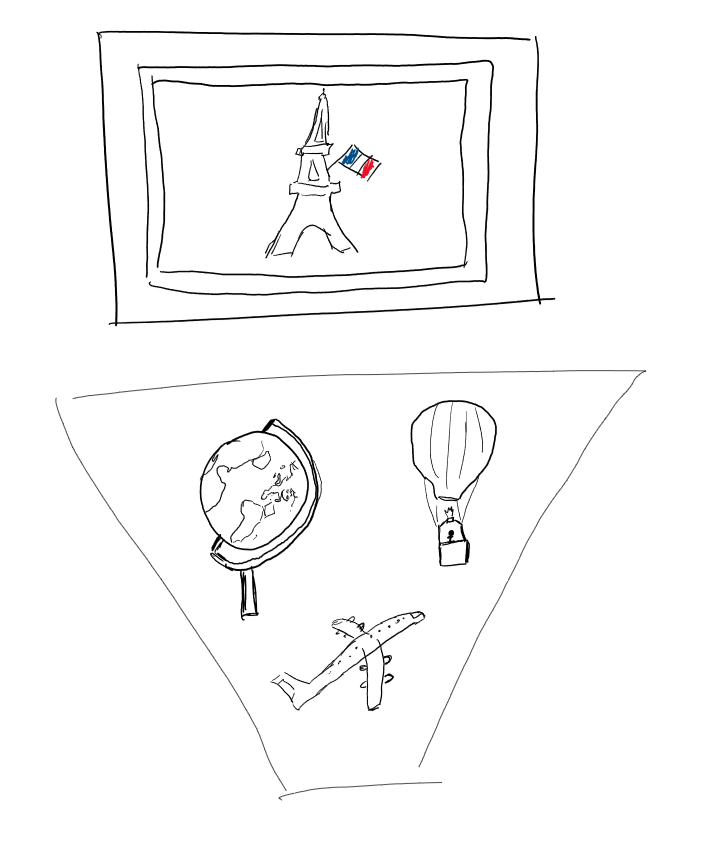
\includegraphics[width=0.5\textwidth]{03.EstudioProblema/02.AnalisisInicial/00.Figuras/03.turismo.png}
    \caption{Boceto de la prueba de turismo. Se presenta una imagen de la torre Eiffel con decorado extra al frente.}
    \label{fig:AI_turismo}
\end{figure}


\subsection{Lenguaje}

Esta categoría se centra en entrenar el razonamiento y el habla del usuario. Para ello se presentarán imágenes que para que el jugador piense y hable sobre lo que sucede en ellas, posiblemente también activando la memoria del usuario en caso de que haya experimentado una situación similar.

\subsubsection{Situaciones}

En esta prueba el estímulo visual que recibe el jugador son imágenes de situaciones cotidianas con las que el jugador pueda, posiblemente, identificarse. Se intenta hacer que el usuario hable y desarrolle un tema lo máximo posible, pudiendo incluso responder preguntas sobre la situación planteada. Por esto, las imágenes deben representar situaciones habituales o claramente reconocibles, pero intentando mantener un valor emocional que pueda despertar recuerdo en el usuario, entrenando así su memoria, dando pie a más desarrollo por su parte e incluso a revivir ciertas sensaciones y sentimientos.


\subsubsection{Descripciones}

Está prueba es análoga a la anterior, pero intentando llevar el proceso a la inversa. En este caso se presentarán una serie de descripciones textuales al usuario, a partir de las cuales él deberá inferir qué está sucediendo en la hipotética situación. Por ejemplo, se pueden describir el aspecto de personas o cómo van vestidas, qué objetos se encuentran al rededor, o qué se puede oír en la escena. De este modo se puede entrenar no solo la capacidad de razonamiento y las habilidades cognitivas de la prueba anterior, si no también se practica la lectura y la comprensión lectora.




\subsection{Razonamiento}

Las pruebas de esta categoría se centran en entrenar el razonamiento y la percepción de objetos y sonidos. Estás pruebas utilizan de forma más prominente elementos de realidad virtual, presentando al usuario objetos tridimensionales con los que puede y debe interactuar. El jugador puede coger, mover y observar de cerca cualquier objeto de estas pruebas. Se busca así alimentar la curiosidad del jugador y potenciar su razonamiento sobre los objetos que tiene a su disposición.

\subsubsection{Agrupación de objetos}

Delante del jugador aparecen una serie de objetos modelados en 3D (véase figura \ref{fig:AI_agrupacion}). Estos objetos son completamente interactivos y el jugador tiene que intentar clasificarlos en dos categorías. Las categorías serán fijas para cada prueba, pero el jugador no las conocerá, por lo que tendrá que razonar para encontrar una conexión entre dos pares de objetos. 

Es importante que los objetos elegidos representen su categoría de forma inequívoca y que habiendo presentes dos objetos de una misma categoría, su conexión sea aparente. Una vez el jugador descubra cuales son las dos categorías ocultas y qué par de objetos pertenece a cada una, deberá coger los objetos virtuales y moverlos para posicionarlos en una zona determinada para cada categoría. 

\begin{figure}
  \centering
    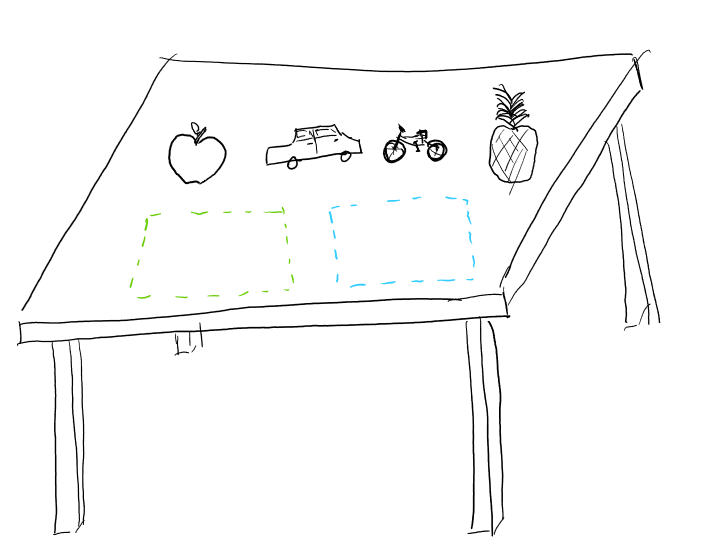
\includegraphics[width=0.5\textwidth]{03.EstudioProblema/02.AnalisisInicial/00.Figuras/04.agrupacion_objetos.png}
    \caption{Boceto para la prueba de asociación de objetos, mostrando dos zonas (verde y azul) para la clasificación de los objetos.}
    \label{fig:AI_agrupacion}
\end{figure}

\subsubsection{Asociación de sonidos}

En esta prueba se presentan al jugador cuatro objetos virtuales de la misma forma que en la prueba anterior, pero en este caso no tendrá que clasificarlos. Todos los objetos representarán análogos del mundo real que produzcan sonidos fácilmente reconocibles. A continuación, se reproduce para el usuario el sonido característico de uno de los objetos que tiene delante. El jugador tendrá que razonar y recordar de sus experiencias en la vida real cuál de los objetos es el que produce el sonido que está escuchando. Cuando está seguro de su respuesta, el jugador coge el objeto virtual y lo selecciona como su respuesta.




\subsection{Comprensión espacial}

En esta última categoría se intenta usar las ventajas de la realidad virtual para entrenar la comprensión espacial del usuario. Gracias a la RV el jugador puede moverse libremente dentro del espacio de juego, coger y mover objetos virtuales, y observarlos de cerca, todo ello con una curiosidad despertada por el formato de la RV que es uno al que la mayoría de los jugadores no estarán acostumbrados. Utilizando estas características se han diseñados dos pruebas que son especialmente efectivas en RV por su grado de inmersión y las posibilidades que ofrece y que, de intentar imitarlas en la vida real, no serían tan efectivas o romperían la inmersión en el entrenamiento cognitivo.

\subsubsection{Figuras superpuestas}

En esta prueba se presentan al jugador varias siluetas oscurecidas, posiblemente de objetos tridimensionales usados en otras pruebas, para que se trate de descubrir de qué objeto se trata en cada caso. También se pueden presentar objetos no oscurecidos, pero superpuestos visualmente unos con otros. El jugador tiene que entender la posición que ocupa cada objeto en el espacio, separándolos mentalmente para descubrir qué objetos son los que tiene delante.


\subsubsection{Localización de sonidos}


Las personas tienen dos oídos, uno a cada lado de la cabeza, lo que produce ligeras diferencias en el sonido que capta cada uno. Este comportamiento es análogo al de la vista, en el cual se basa toda la realidad virtual (véase párrafo sobre la visión estereoscópica en el apartado \ref{par:estadoArte:estereoscopio}). Por ello, las personas son capaces de distinguir la procedencia de un sonido incluso con los ojos cerrados. Durante mucho tiempo no se ha dado importancia a esta faceta del audio digital, pero con el auge de la RV es cada vez más común que videojuegos utilicen audio espacializado digitalmente para imitar el comportamiento del mundo real. Unity soporta este tipo de audio, por lo que se puede crear una prueba que lo aproveche y sea capaz de entrenar la comprensión espacial del jugador. Durante esta prueba, se coloca una fuente de sonido espacializado en algún punto al rededor del usuario (vease figura \ref{fig:AI_localizacionSonido}), y este será capaz de percibir desde que punto proviene el sonido. Para superar la prueba el jugador debe descubrir dónde se encuentra la fuente sonora y girarse para mirarla de frente.

\begin{figure}
  \centering
    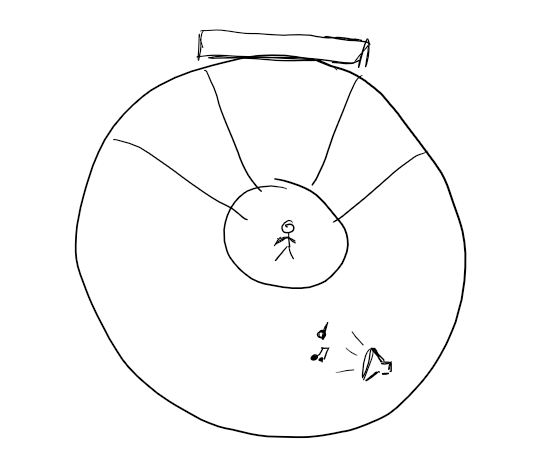
\includegraphics[width=0.5\textwidth]{03.EstudioProblema/02.AnalisisInicial/00.Figuras/05.localizacion_sonido.png}
    \caption{Boceto de la vista cenital del escenario principal, mostrando una posible colocación de la fuente de sonido para la prueba de localización de sonidos.}
    \label{fig:AI_localizacionSonido}
\end{figure}

\section{Desarrollo}


Antes de comenzar el juego, se presentará al usuario una pantalla en la que podrá elegir ciertos parámetros para el juego y que servirán para adaptar la sesión de juego al jugador concreto. Estas opciones ajustan el tipo de pruebas que pueden aparecer o no durante la partida, el número de rondas a jugar, si el jugador estará sentado o de pie, si tiene alguna dificultad auditiva o motora, o si la realización de las pruebas otorgará puntos, entre otros parámetros. El objetivo de esta pantalla de configuración es poder crear la mejor experiencia de juego posible para cada usuario.

A continuación, el juego dará comienzo y el jugador aparecerá en un entorno virtual ambientado en un plató de televisión donde se realizará la introducción al juego. Una vez todo listo dará comienzo la primera ronda del concurso. Todas las rondas siguen la misma estructura:


\begin{itemize}
	\item{Primero se presentarán al jugador dos pruebas diferentes y este podrá elegir a cuál de ellas va a enfrentarse en la ronda.}

	\item{A continuación, el jugador será transportado a un nuevo entorno propiamente ambientado para la prueba que ha elegido. Cuando esté listo, comenzará la prueba.}

	\item{Si las puntuaciones están activas, el jugador recibirá una puntuación a corte a su ejecución en la prueba siempre que sea posible cuantificar dicha ejecución.}
	
	\item{Finalmente, el jugador es transportado de vuelta a escenario de juego principal y la ronda finaliza.}

\end{itemize}

Tras la finalización de la última ronda, se realiza un recuento de puntos si procede, se muestra un resumen de las actividades realizadas y se da por terminada la sesión de juego.


Este juego estará diseñado para que pueda ser utilizado por una persona de manera individual, pero también permitirá la interacción de una persona externa al entorno virtual. Esta persona actuará como ayudante del jugador, pudiendo cambiar el comportamiento del juego saltando pruebas, evaluando y puntuando las mismas o simplemente guiando al jugador, que puede verse descolocado en el entorno virtual. Además, por la naturaleza de algunas de las pruebas, se requiere de la interactuación y evaluación de una persona con los conocimientos adecuados en entrenamiento cognitivo. De esta manera se ofrece este videojuego como una herramienta para que profesionales puedan animar a las personas que reciben entrenamiento cognitivo y hacerlo más llevadero y entretenido.

\chapterend